
\section{Case Definitions}

The paper focuses on the benefits that arise from the strategic siting of a repository 
on a non-operating nuclear facility, and not the benefits that arise from the repository design. 
The borehole design follows the Sandia Report Reference Design and Operations 
for Deep Borehole Radioactive Waste \cite{arnold_reference_2011}. Selection of 
an alternative borehole concept could impact the details of the repacking needs 
and facility design, but will not significantly impact the siting comparison 
in this paper.
 
\subsection{Case I: Reference Case} 
The reference case, upon which the proposed case seeks to improve, is to build 
a standalone 70,000 \gls{MTHM} mined repository at the Yucca Mountain site.

The reference case is presented in order to demonstrate the cost savings and efficiencies 
that arise from the proposed case. The base case mimics the Yucca Mountain Project.
Costs include new licensing and processing facility for repacking the spent fuel assemblies.

\subsection{Case II: Shut Down Plant Case}

The imminent shutdown of the Clinton Nuclear Power Station has recently been 
averted by an act of the state legislature. In this sense, Clinton is 
representative of a class of at-risk nuclear 
reactors in the Midwest and eastern United States. A borehole repository 
sited at the Clinton Nuclear Power station site is therefore hypothetically 
considered here to represent integrated repository siting at a reactor facility 
faced with potential shutdown.

The Clinton Nuclear Power Station is owned by the Exelon Corporation. It has a 
licensed land area of approximately $58 km^2$ and a $20 km^2$ cooling heat sink, 
the Clinton Lake. Of the licensed land area, only $0.6 km^2$ is used for the facility.  
\cite{nrc_chapter_2007}.  This leaves enough room left for a 70,000 \gls{MTHM} 
borehole repository without additional land purchase from the public.


\section{Methodology}

This work will evaluate \textbf{2 scenarios} for repository siting according to \textbf{6 metrics} of 
performance considered from the perspective of \textbf{4 stakeholders.}

This work will evaluate the potential impacts of each siting strategy according 
to the following 6 quantitative measures:

\begin{itemize}
	\item Transportation Burden $[MTHM \cdot km]$: A site is preferred by 
	most stakeholders if it can minimize the distance \gls{SNF} 
	must travel.
	\item Workforce Utilization $[-]$: A repository site is preferred by 
	many stakeholders if it utilizes an already situated skilled local 
	workforce. 
	\item Expediency $[y]$: Many stakeholders will benefit if the removal 
	of dry casks from current storage pads is expedited.
	\item Consent Basis $[\frac{nuclear MW}{\mbox{capita}}]$: If the community
	 beneifts from nuclear energy, they are more likely to be consenting to
	 site a repository. If there is a basis for a consent-based 
	siting process to succeed, many stakeholders benefit.
	\item Site Access $[-]$: Rail access to the site is essential for 
	beginning operations.
	\item Site Appropriateness $[-]$: A site must be geologically 
	appropriate and of sufficient area.
\end{itemize}

Finally, recognizing that these measures are valued differently by each, we
consider possible weighting factors that may capture the perspectives of 4 key
stakeholder groups:

\begin{itemize}
	\item the federal government,
	\item the state government,
	\item the local government / community,
	\item and the owner of the non-operating plant.
\end{itemize}


\section{Evaluation Metrics}

This paper introduces six metrics of siting performance. These metrics and 
their definitions draw upon previous 
\cite{freeze_siting_2015,waleed_regional_2015} as well as original work.  In 
the following sections, the metrics are defined in more detail, and normalized
so that in the final section, they are applied to comparatively evaluate each case.

The normalization of the metrics are done to a scale of 0 to 1 using the equation
below, where 0 is the worst possible value, and 1 the best. 
 Metrics like transportation burden, expediency, and consent basis,
 are normalized in such a matter. Metrics without units are booleans, where values 
 only exist in values of 0 or 1. For example, a 0 value for site access means 
that there is no existing site access infrastructure.


\begin{align} 
	\mbox{NV} &= \frac{x-\mbox{W}}{\mbox{B}-\mbox{W}}\\
	NV &= \mbox{normalized value for the metric}\\
	x &= \mbox{considered case value for the metric}\\
	B &= \mbox{best case value for the metric}\\
	W &= \mbox{worst case value for the metric}\\
\end{align}



\subsection{Transportation Burden}
 A metric 
 for representing the distance a mass of spent fuel must be transported, the 
 transport burden, is introduced. This transportation burden is the product 
 of the \gls{SNF} mass and the distance it has to travel from its current 
 storage location to the proposed repository. This results in a 
 metric in units of $MTHM\cdot km$. 

 To arrive at the transportation burden for each case, a distance analysis was 
 completed using the Haversine formula \cite{shumaker_astronomical_1984}. 
 First, the coordinates of each power plant were obtained by scraping public 
 data \cite{nuclear_regulatory_commission_nrc:_2016}.  The distance between each storage site (i.e. reactors 
 and \gls{ISFSI}) was then calculated by using the Haversine formula on the 
 geographical coordinates of the receiving and sending sites (1 and 2). 

This analysis used GC-859 spent fuel inventory data available from \gls{EIA} 
through private communication \cite{domenico_GC-859_2016} as well as \gls{CURIE}, a web interface to 
the \gls{ORNL} universal database\cite{ornl_centralized_2016}.
From the list of 74 sites, several candidates which minimize $B [MTHM\cdot 
km]$, spent fuel transportation burden, are listed in Table 1.
    
    \begin{table}[h]
    	\centering
    	
    	\caption {Reactors with relatively small spent fuel transportation burden $ [MTHM\cdot km]$.}
    	\scalebox{0.86}{
    		\begin{tabular}{|c|c|c|c|}
    			\hline
    			Reactor & State & $MTHM*km$ & License Area [$km^2$]  \\ \hline
    			Clinton & Illinois &  \textbf{77,352,339} & \textbf{57.87}   \\ \hline
    			Dresden & Illinois &  \textbf{77,663,969} & 3.856   \\ \hline
    			Peach Bottom & Pennsylvania & 85,563,135 & 2.509   \\ \hline
    			Indian Point &   New York & 84,097,374 & .967   \\ \hline
    			Yucca Mountain & Nevada & 209,575,157 & N/A \\ \hline
    			
    		\end{tabular}}
    		\end {table}

The Clinton Power Plant was chosen as the site for the proposed case due to its
small $MTHM\cdot km$ value and substantially large license 
area\cite{nrc_chapter_2007}.



\begin{table}[h]
	\centering
        \caption {Transportation Burden for Each Case}
	%\scalebox{0.60}{
		\begin{tabular}{|c|c|c|}
			\hline
			Case & Transportation Burden [$MTHM\cdot km$] & NV\\
			\hline
			Case I & 209,575,157  & 0\\
			Case II & 77,352,339 & 1 \\
                        \hline
                \end{tabular}
                %}
\end{table}
  

 \subsection{Site Appropriateness} 

  To host a borehole repository, the site must satisfy geologic requirements. 
  Figure \ref{fig:cbrock} is a map indicating the geological fitness of various 
  regions of the United States. The proposed site at Clinton sits above 
  a crystalline basement which lies at an appropriate depth.

\begin{figure}[!h] 
  \centering
  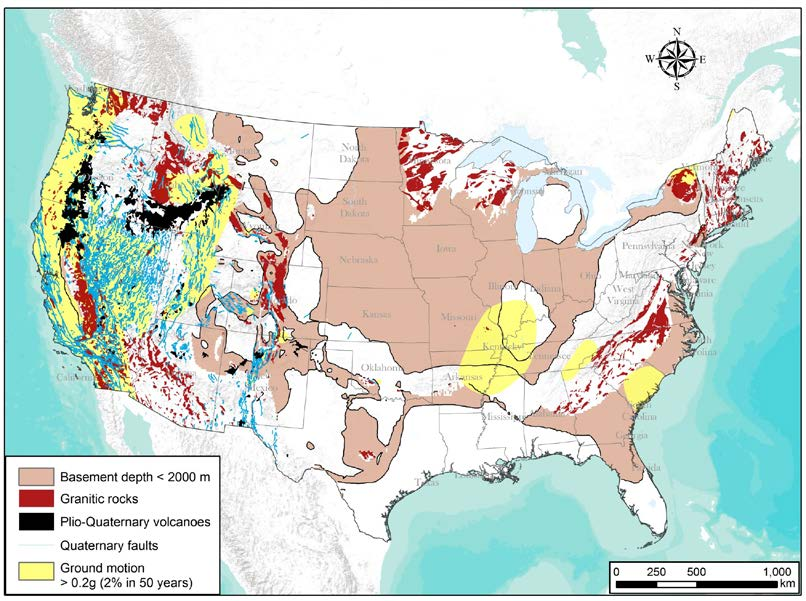
\includegraphics[width=0.8\columnwidth]{cbrock.png}	
        \caption{From \cite{perry_gis_2015}, a map of areas in the US with 
        crystalline basement rock at less than 2000 meters depth. Tectonic 
        activity impacting siting considerations are also mapped:  Quaternary 
        faulting, volcanism, and seismic hazard (yellow shading = 2\% 
        probability of exceeding 0.2 g of ground acceleration in 50 years).}
  \label{fig:cbrock}
\end{figure}
 
  
\begin{table}[h]
	\centering
        \caption {Site Appropriateness for Each Case}
	%\scalebox{0.60}{
		\begin{tabular}{|c|c|}
			\hline
			Case & Site Appropriateness \\
			\hline
			Case I & 1 \\
			Case II & 1 \\
			\hline
                \end{tabular}
                %}
\end{table}

\subsection{Workforce Utilization}

The Clinton
 Power Station has approximately 700 employees living in nearby counties with an
additional several hundred contractors during fuel 
outages\cite{exelon_clinton_2016}.
The existing skilled workers and local talent for maintenance, transport and catering
services can be utilized without bringing a whole new group of workers to the 
area \cite{iaea_managing_2008}. Also, the shutdown of Clinton Power Plant would cause a dramatic
loss of jobs in the community. 

The proposed case has a larger advantage over the base case in the sense that there
are already existing facility in regards to spent fuel handling and worker lodging 
and catering services. 
It is assumed, for the sake of argument, half of the construction cost of the
repacking facility in the base case is used to expand the existing facility in the
proposed case. 


\begin{table}[h]
	\centering
        \caption {Workforce Utilization for Each Case}
	%\scalebox{0.60}{
		\begin{tabular}{|c|c|}
			\hline
			Case & Workforce Utilization \\
			\hline
			Case I & 0 \\
			Case II & 1 \\
			\hline
                \end{tabular}
                %}
\end{table}


\subsection{Consent Basis}

International \gls{SNF} siting experiences have shown that a consent-based
approach to siting a repository is crucial to success
\cite{ayers_blue_2012,doe_designing_2016,jenkins-smith_public_2013,freeze_siting_2015}. 
Furthermore, the Swedish precedent \cite{olsson_experiences_2013} shows that 
municipalities near nuclear facilities
are more likely to volunteer to site a repository in their community.

Because populations local to operating reactor sites are more likely to be 
favorable toward nuclear power, and the proposed integrated siting 
is in an already-nuclear community by design, this siting strategy inherently 
maximizes the local consent basis.

The source of this favorable attitude varies by site. 
The local community is the beneficiary of various economic benefits
including job creation and the substantial property taxes paid by the utility 
toward regional governmental budgets.   In the case of the Clinton Power Plant, 
Exelon pays \$15 million in property taxes each year, which amounts to about 
\$923 per resident in the host Dewitt county \cite{brady-lunny_dewitt_2016}. The plant
also provides a total payroll of more than \$50 million to its workers.
The eventual shutdown of the plant would have caused a dramatic loss of the economic inflow.
It is also speculated that 13,300 jobs would be lost in Illinois after five years 
of plant shutdown \cite{reid_study:_2014}.  

A similar phenomenon might be expected at the state level as well, because 
Illinois generates more nuclear energy than any other U.S.  state with a net 
capacity of 11,441 megawatts in 2010 \cite{eia_state_2012}. Nevada, on the other 
hand, hosts zero nuclear power plants. Thus, it can only be natural for Nevada 
to consider a national repository as an unjust burden, despite economic 
benefits.  

The consent basis, driven by proximity to an operating nuclear plant and 
corresponding greater likelihood to be favorable toward hosting an \gls{SNF} 
repository, should be quantifiable by a measure of the benefit experienced by 
the community.  For simplicity, we quantify the proximity to nuclear energy at 
the state level  based on power consumed. The corresponding state and regional 
metrics (expressed in MW of nuclear power per capita) are listed in Table V. This 
analysis uses nuclear power generation capacity and population data from the 
U.S. \gls{EIA} \cite{eia_state_2012} and the U.S. Census \cite{census}.  

\begin{table}[h]
	
	\centering
	\caption {\gls{NMWPC} values for different states}

	\scalebox{0.60}{
		\begin{tabular}{|c|c|c|c|c|}
			\hline
			State & Net Nuclear Capacity (MW) & Census Population & \gls{NMWPC} ($10^{-3}$) \\ \hline
			South Carolina & 6,486 & 4,625,401 & 1.4  \\ \hline
			Alabama & 5,043 & 4,780,127 & 1.05 \\ \hline
			Vermont & 620 & 625,745 & .99 \\ \hline
			Illinois & 11,441 & 12,831,549 & .89 \\ \hline
			Nevada & 0 & 2,705,000 & 0 \\ \hline
			Average Nuclear States & 101,167 & 265,386,569 & .38 \\ \hline
			Average National & 101,167 & 309,300,000 & .33 \\ \hline
			
		\end{tabular}
        }
	\end{table}
	
The state of Illinois has the highest generating capacity, and is fifth in the \gls{NMWPC}
 value, while Nevada has zero generating capacity with zero MW per capita value. 
Illinois' \gls{NMWPC} value is also well above the national average. Judging from the
table, it is no surprise that the state of Nevada rejected the idea of having a national
spent fuel repository on its land. On the other hand, Illinois is more familiar with 
nuclear and also somewhat reliant on nuclear, which can lead to a consent-based process
in a state-level. 

\begin{table}[h]
	
	\centering
	\caption {\gls{NMWPC} values for Each Case}

		\begin{tabular}{|c|c|c|}
			\hline
			Case & NMWPC & NV \\
			\hline
			Case I & 0 & 0\\
			Case II & .89 & .635\\
					\hline
                \end{tabular}
                %}
\end{table}


\subsection{Site Access}

Site access necessary to transport radioactive material to the repository site 
poses one of the greatest logistical challenges in siting a repository. 

In the case of Yucca Mountain, 
the opposition from the state of Nevada to the proposed Caliente rail corridor 
blocked construction of the rail line and indefinitely postponed
acceptance of \gls{SNF} at Yucca Mountain \cite{halstead_yucca_2011}.

Operating reactors, conversely, are much more likely to be located along rail 
lines. In the case of the Clinton nuclear power plant, 
the Canadian National rail line \cite{waleed_regional_2015} has a station in 
Clinton and dedicated tracks leading into the reactor facility, as shown in 
Figure \ref{fig:cnmap}. An already existing railway can avoid costs and delays related
 to building a new infrastructure.

\begin{figure}[!h] 
  \centering
  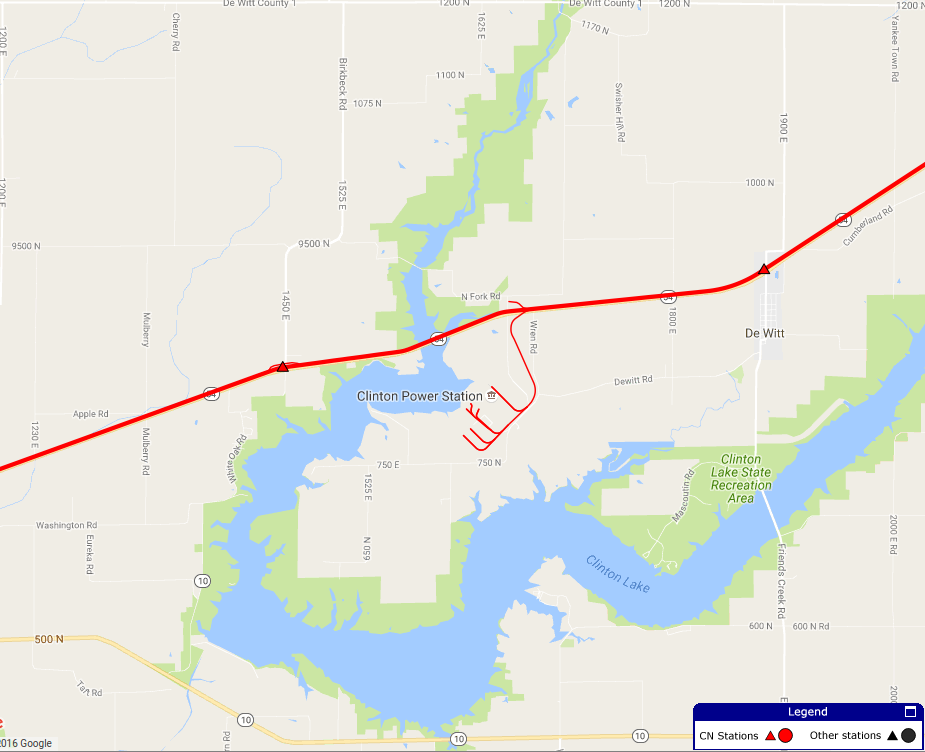
\includegraphics[width=0.8\columnwidth]{cnmap.png}	
        \caption{From \cite{canadian_national_railway_company_canadian_2016}, a map of Clinton Power Station in Clinton,IL
        with the Canadian National rail passing through.}
  \label{fig:cnmap}
\end{figure}

The proposed site's proximity to other power plants means that the transport
routes pass through fewer states and communities, which lessens the potential 
for conflict.


\begin{table}[h]
	\centering
        \caption {Site Access for Each Case}
	%\scalebox{0.60}{
		\begin{tabular}{|c|c|}
			\hline
			Case & Site Access \\
			\hline
			Case I & 0 \\
			Case II & 1 \\
			\hline
                \end{tabular}
                %}
\end{table}



\subsection{Expediency}

Leveraging existing infrastructure at an integrated site will allow for 
expedited acceptance of \gls{SNF} from temporary dry cask storage sites 
nationwide.

Dry casks are the result of the perpetual delay of a repository construction.
The proposed case would allow reactor sites to empty their spent fuel pools, which
would no longer necessitate dry storage campaigns. For example, Maine Yankee's 
\gls{ISFSI} cost was \$149.3 million in 2001 dollars, with an annual operating fee
of \$10 million per year \cite{lee_costing_2009}. 

The proposed case, once completed, will allow faster acceptance of \gls{SNF} and, 
accordingly, resumed collection of the \gls{NWF}, 
which will fund the repository operation and maintenance.

The proposed case, being a once-operating nuclear power plant, has the facility to 
repack the spent fuel assemblies into a disposal cask. Its dry cask infrastructure 
is currently in use. However, this facility needs to be upgraded to increase its throughput, and should be preferably automatic, to minimize worker exposure. The transported spent fuel assemblies are repacked and inspected at the upgraded facility, and is sent to the emplacement tubes for final disposal. Not having to build an entirely new above-ground facility should greatly ease the consent-based process, for it seems like there would be minimal impact. 
 
A metric for expediency is then proposed which is inversely proportionate to 
the number of years until the federal government takes possession of the spent 
fuel. Estimating the likely timelines for each case is a challenge beyond the 
scope of this work. However, a bounding estimate can be derived from the time 
saved from use of existing infrastructure at the integrated facility. Avoiding 
that handling facility delay will save at least 5 years 
and likely much more on the timeline of Case II over that of Case I 
\cite{doe_strategy_2013}. 

\begin{table}[h]
	\centering
        \caption {Expediency in Each Case}
	%\scalebox{0.60}{
		\begin{tabular}{|c|c|c|}
			\hline
                        Case & Time Saved [y] & NV \\
			\hline
			Case I & 0 & 0\\
			Case II & 5 & 1 \\
			\hline
                \end{tabular}
                %}
\end{table}

\section{Results and Discussion} 

To model the impact of these measures on the incentives of each stakeholder, 
the list of stakeholders considered follows in Table \ref{tab:stakeholders} 
alongside the weights indicating the magnitude of the importance of the incentive.
 
\begin{table}[h]
\centering
\caption {Metrics and Weight for Each Stakeholder}
\label{tab:stakeholders}
\scalebox{0.8}{
	\begin{tabular}{|l|c|c|c|c|}
	\hline
	Metric & Federal & State & Local & Utility  \\ \hline
	Transportation Burden & 3 & 2 & 1 & 1    \\ \hline
	Site Appropriateness & 3 & 2 & 1 & 1 \\ \hline
	Workforce Utilization & 3 & 2 & 2 & 2 \\ \hline
	Consenting Locals & 3 & 2 & 3 & 2 \\ \hline
	Site Access & 3 & 2 & 1 & 1 \\ \hline
	Expediency & 3 & 2 & 1 & 3 \\ \hline \hline
	Case I total & 3 &2 &1 & 1 \\ \hline
	Case II total & 16.9 & 11.2 & 7.9 & 9.2 \\ \hline
	\end{tabular}}
\end{table}

Results show that it is far more attractive for various stakeholders to 
site a repository at a non-operating nuclear power plant. Through strategical
siting, all the parties involved can benefit.

Given the current circumstances, a repository is crucial for the survival of nuclear
power. By siting one in a central location with sufficient licensed land,
a repository with sizable capacity can be built cheaper, more efficiently, and 
in a consent-based manner with the local community. 
